% Style template ines (july 2015)
\documentclass[ngerman]{zhawines}

% Include
\usepackage[utf8]{inputenc}
\usepackage[ngerman]{babel}
\usepackage{scrpage2}
\usepackage{listings}
\usepackage{amsmath}
\usepackage[squaren]{SIunits}
\usepackage{graphicx}
\usepackage{array}
\usepackage{todonotes}
\usepackage{float}
\usepackage[toc,page]{appendix}
%\usepackage[autostyle=true,german=swiss]{csquotes} % quotes
%\usepackage[nottoc]{tocbibind}
\usepackage[sectionbib]{natbib} % bibl will be a section and not a chapter
\bibliographystyle{abbrvnat}
\setcitestyle{authoryear,open={(},close={)}}
\usepackage[justification=raggedright,singlelinecheck=false]{caption}
\usepackage{helvet}

\usepackage[pdfauthor={Katrin Bächli}, pdftitle={Projektarbeit HS15 Studiengang Elektrotechnik - Polyphonic DDS Synthesizer mit MIDI Steuerung}, colorlinks=true,linkcolor=black,urlcolor=black,citecolor=black,plainpages=false]{hyperref}


% \usepackage[latin1]{inputenc}    %Umlaute  -> Fehler: "option clash for package inputenc

%\renewcommand{\contentsname}{Inhaltsverzeichnis}

%---------------------------------------------------------------------
\begin{document}

	\hbadness 10000
	\author{Katrin Bächli }%  -> Fehler: Error: unicode char \u8:äch not set up for use with LaTeX \maketitle
	\renewcommand{\betreuer}{Prof. Hans-Joachim Gelke}
	\renewcommand{\nebenbetreuer}{Dr. Matthias Rosenthal}
	\title{Polyphonic DDS Synthesizer\\ mit MIDI Steuerung}
	\subtitle{PA15\_gelk\_1}
	\email{katrin.baechli@zhaw.ch}


	\maketitle{}
	
	\headings
	
	
	%%%%%%%%%%%%%%%%%%%%%%%%%%%%%%%%%%%%%%%%%%%%%%%%%%%%%%%%%%%%%%%%%
%  _____       ______   ____									%
% |_   _|     |  ____|/ ____|  Institute of Embedded Systems	%
%   | |  _ __ | |__  | (___    Wireless Group					%
%   | | | '_ \|  __|  \___ \   Zuercher Hochschule Winterthur	%
%  _| |_| | | | |____ ____) |  (University of Applied Sciences)	%
% |_____|_| |_|______|_____/   8401 Winterthur, Switzerland		%
%																%
%%%%%%%%%%%%%%%%%%%%%%%%%%%%%%%%%%%%%%%%%%%%%%%%%%%%%%%%%%%%%%%%%

\chapter*{Zusammenfassung}

Der erste Teil der Projektarbeit befasst sich mit zwei Herausforderungen der hardwarenahen Sprache VHDL. 

Als Erstes werden sogenannte \textit{glitches}, ungewollte Signalspitzen, künstlich herbeigeführt. Dies geschieht, in dem man die Signalpfade über externes Routing verlängert und dadurch der logische Wert verzögert beim nächsten Bautei, einem \textit{decoder}, eintrifft. Wird der \textit{decoder} asynchron betrieben, so verarbeitet dieser kurzzeitig falsche Werte, was in einem \textit{glitch} sichtbar gemacht wird. 

Als Zweites wird in einer Schaltung ein metastabiler Zustand provoziert. Damit dies erreicht wird, muss die \textit{hold} - oder die\textit{ setup time} eines Flip-Flops verletzt werden. Erzeugt wird die Metastabilität durch unterschiedliches Takten zweier Logiken. Der Ausgang der ersten \textit{clock domain} wird als asynchron Inpuls auf eine \textit{finate state machine} einer anderen \textit{clock domain} geführt. Die \textit{finate state machine} fällt nach kürzester Zeit in einen undefinierten Zustand, einen Zustand, den sie nicht implementiert hat.



Der zweiten Teil der Projektarbeit beinhaltet das Entwickeln eines polyphonen \textit{midi interface} für das Synthesizer-Projektes der Vorlesung Digitaltechnik II. Gemäss dem MIDI 1.0 Standard wird ein Controller implementiert, der auch das Drücken mehrer Tasten zuverlässig detektiert. Um die Entwicklung effizient zu gestalten, wird von Beginn weg mit einer textbasierten \textit{testbench} gearbeitet. 
Für die Ausgabe der maxibal 10 gleichzeitig ertönenden Noten wird ein zweiter Block für das Händeln der ein und aus der einzelnen NOten geschrieben. Beide Blocks sind eingehend mit der testbench getestet und deren Verhalten gut dokumentiert.

(weglassen ??? Erst am Schluss nennen.... )
Als offener Punkt besteht die Implementation des \textit{midi interfaces} in das bestehende Synthesizer-Projekt. Die Schnittstellen sind im Anhang festgehalten und die notewnigen Implementationsschritte, wie das Ausweiten des bestehenden DDS auf 10 DDS sind im Projekt als Blöcke eingebaut. Aus zeitlichen Gründen konnte dieser letzte Schritt nicht mehr während der Projektarbeit zu Ende gebracht werden. 


		
	%%%%%%%%%%%%%%%%%%%%%%%%%%%%%%%%%%%%%%%%%%%%%%%%%%%%%%%%%%%%%%%%%
%  _____       ______   ____									%
% |_   _|     |  ____|/ ____|  Institute of Embedded Systems	%
%   | |  _ __ | |__  | (___    Wireless Group					%
%   | | | '_ \|  __|  \___ \   Zuercher Hochschule Winterthur	%
%  _| |_| | | | |____ ____) |  (University of Applied Sciences)	%
% |_____|_| |_|______|_____/   8401 Winterthur, Switzerland		%
%																%
%%%%%%%%%%%%%%%%%%%%%%%%%%%%%%%%%%%%%%%%%%%%%%%%%%%%%%%%%%%%%%%%%

\chapter*{Abstract}\label{chap.abstract}

An important part in digital signal processing is the hardware-related programming language VHDL. In this thesis, two independent tasks have been drawn up and implemented using VHDL.

On the one hand was the inducing of hardware-related glitches and metastability, and on the other hand the implementation of a MIDI-interface, whose development is built on a text-based testbench.

By extending the paths of individual signals on a Cyclone II-FPGA it is possible to generate artificial glitches. Hence, some signals arrive delayed at the asynchronous decoder. Wrong information will be processed and put on the signal lines, which occurs in so-called glitch.

Metastable states are caused by clocking two VHDL logic blocks with two independent clocks, where no clock is a multiple of the other one. The output signal of the first block is connected as a asynchronous input of the second block. Since the two blocks work in a different clock domain, the finite state machine can fall in undefined state, in other words the finite state machine is in a metastable state.

--- letzter Teil fehlt... 		
	%%%%%%%%%%%%%%%%%%%%%%%%%%%%%%%%%%%%%%%%%%%%%%%%%%%%%%%%%%%%%%%%%
%  _____       ______   ____									%
% |_   _|     |  ____|/ ____|  Institute of Embedded Systems	%
%   | |  _ __ | |__  | (___    Wireless Group					%
%   | | | '_ \|  __|  \___ \   Zuercher Hochschule Winterthur	%
%  _| |_| | | | |____ ____) |  (University of Applied Sciences)	%
% |_____|_| |_|______|_____/   8401 Winterthur, Switzerland		%
%																%
%%%%%%%%%%%%%%%%%%%%%%%%%%%%%%%%%%%%%%%%%%%%%%%%%%%%%%%%%%%%%%%%%

\chapter*{Vorwort}\label{chap.vorwort}
an Alexey: Bitte hier auf inhaltliche Richtigkeit prüfen. Brauche es erst am Do
korrekt ...

Meine Motivation ist das vertiefte Kennenlernen der Sprache VHDL. Diese hardwarenahe Sprache beinhaltet mit der kombinatorischen Logik und der auch nicht sequentiellen Prozessverarbeitung Eigenheiten, mit denen ich Umgehen lernen wollte.

In der Projektarbeit waren es exakt diese Punkte, mit denen ich viel Zeit durch Debuggen verbrachte. Doch gerade so, ist mir nun diese Art der Programmierung vertrauter geworden und ich freue mich, auf kommende VHDL-Projekte.

Ich möchte Prof. Hans-Joachim Gelke meinen Dank aussprechen. Er legte den Fokus immer wieder auf die kombinatorische Logik und die Konsequenz des Codes, für das Umsetzen in der Hardware. Ebenfalls möchte ich Dr. Matthias Rosenthal danken, der diskret im Hintergrund die Arbeit mittrug und den Entwicklungsprozess mittrug.

Ich denke, dass diese Arbeit vor allem für Software Ingenieure interessant ist, da sie einen groben Einblick in die hardwarenahe Programmierung erhalten.

(Name ???)
(Ort???)
(Datum ??)\\


	
	
	
	% Inhaltsverzeichnis	
	\tableofcontents				
	%%%%%%%%%%%%%%%%%%%%%%%%%%%%%%%%%%%%%%%%%%%%%%%%%%%%%%%%%%%%%%%%%
%  _____       ______   ____									%
% |_   _|     |  ____|/ ____|  Institute of Embedded Systems	%
%   | |  _ __ | |__  | (___    Wireless Group					%
%   | | | '_ \|  __|  \___ \   Zuercher Hochschule Winterthur	%
%  _| |_| | | | |____ ____) |  (University of Applied Sciences)	%
% |_____|_| |_|______|_____/   8401 Winterthur, Switzerland		%
%																%
%%%%%%%%%%%%%%%%%%%%%%%%%%%%%%%%%%%%%%%%%%%%%%%%%%%%%%%%%%%%%%%%%

\chapter{Einleitung}\label{chap.einleitung}

\section{Ausgangslage}\label{sect.einleitung_ausgangslage}

Für den ersten Teil der Arbeit, die Timing Artifakte  \textit{Glitch} und \textit{Metastability} zu demonstrieren, gibt es wenige Referenzprojekte. Da die Zustände ungewollt sind, finden sie als Fehlerquellen Erwähnung in der Literatur \citep{ReferenceManual}, \citep{F_glitches}, \citep{F_metastability}. Nur ein Dokument wurde gefunden, das die Erzeugung von \textit{Metastability} behandelt \citep{Metastabil}. Aus diesem Grund bezieht sich der Nachweis der Timing Artifakte auf Anregungen und auf die Erfahrung von Prof. Hans-Joachim Gelke.

Im zweiten Teil geht es um den Aufbau eines \textit{MIDI Interfaces}. MIDI bedeutet \textit{Musical Instrument Digital Interface} und ist ein Standard, der die Beschaffenheit der Hardware wie auch das Kommunikationsprotokoll festlegt \citep{Midi_Braut}. Die MIDI Manufacturers Association dokumentiert die mehrfachen Erweiterungen des MIDI 1.0 Standard \citep{Midi_specification}. Diese Spezifikationen bildet die Grundlage für den Block \textit{MIDI Control}. Am Institut for Embedded Systems besteht ein \textit{MIDI UART Top}-Block in VHDL von Armin Weiss. In dieser Projektarbeit zu entwickeln sind die zwei Einheiten \textit{MIDI Control} und \textit{Polyphony Out}. Und anschliessend diese Blocks in das bestehende Synthesizer-Projekt einzubauen. Bei beiden Blocks basiert die Entwicklung auf einer textbasierten Test Bench.

\section{Aufgabenstellung}\label{sect.einleitung_ziele}

Die offizielle Aufgabenstellung befindet sich im Anhang \ref{chap.anhang_aufgabenstellung}. 
 
\begin{itemize}
	\item Erzeugung von Glitches mit einem Zähler und nachgeschaltetem Dekoder. Sichtbarmachung der Glitches mit einem Oszilloskop. Betätigen des asynchronen Resets vom Decoder aus.
	\item Provozieren und sichtbarmachung von metastabilen Zuständen. Hierfür kann z.B. eine Schaltung mit zwei asynchronen externen Takten aufgebaut werden.
\end{itemize}  


Nach Fertigstellen des ersten Teils, wird die Aufgabenstellung für den zweiten Teil präzisiert (siehe Anhang \ref{chap.anhang_aufgabenstellung_neu}).

\begin{itemize}
	\item Midi Interface for Keyboard für Polyphonie nach Konzept von Gelk
	\begin{itemize}
    	\item 10 Frequenz Control Ausgänge zur Steuerung der Tonhöhe des Generators
    	\item 10 On/Off Ausgänge Ton On/Off
    	\item UART wird geliefert von Gelk
   	 	\item VHDL wird von Grund auf neu erstellt.
	\end{itemize}
	\item 10 DDS implementieren und mit Mischer mischen
	\item Script basierte Test Bench. Test Bench erzeugt serielle Midi Daten, so wie sie auf dem DIN Stecker vorkommen (logisch)
	\item Test Bench liest eine Testscript Datei ein, in welcher die Tastendrücke eines Keyboards abgebildet werden können. 
	\item Midi Poliphony Spec muss durch die Test Bench unterstützt werden können. 
	\item Velocity muss nicht unterstützt werden.
	\item Kein VHDL code ohne Test Bench.
	\item Block level Test Bench. Unit Tests.
\end{itemize}
		
	%%%%%%%%%%%%%%%%%%%%%%%%%%%%%%%%%%%%%%%%%%%%%%%%%%%%%%%%%%%%%%%%%
%  _____       ______   ____									%
% |_   _|     |  ____|/ ____|  Institute of Embedded Systems	%
%   | |  _ __ | |__  | (___    Wireless Group					%
%   | | | '_ \|  __|  \___ \   Zuercher Hochschule Winterthur	%
%  _| |_| | | | |____ ____) |  (University of Applied Sciences)	%
% |_____|_| |_|______|_____/   8401 Winterthur, Switzerland		%
%																%
%%%%%%%%%%%%%%%%%%%%%%%%%%%%%%%%%%%%%%%%%%%%%%%%%%%%%%%%%%%%%%%%%

\chapter{Glitches}\label{chap.glitch}

\section{Glitche in der Digitalen Signalverarbeitung}\label{sect.glitch_def}
In der Digitalen Signalverarbeitung ist glitch ein bekannter Fehler, den William I. Fletscher folgendermassen beschreibt: ''Als \textit{glitch}  wird eine ungewollte, flüchtige ''Signalspitze'' bezeichnet, die Zähler aufwärts zählt, Register löscht oder einen ungewollten Prozess startet.'' \cite{F_glitches} \\


Abbildung \ref{fig.glitch.def} zeigt zwei \textit{glitches} in einem Ausgangssignal.\\

\begin{figure}[H]
	\includegraphics[width=\textwidth]{images/glitch/def_glitch_1.png}
	\caption{Zwei Glitches im Ausgangssignal}
	\label{fig.glitch.def}
\end{figure}


\section{Ursache für Glitches}\label{sect.glitch_ursache}
Der Auslöser sind ungleichzeitig eintreffende Signale, die durch \\
1.) unterschiedlich lange Signalpfade, \\
2.) unterschiedliche Durchlaufverzögerungen der vorangehenden Flip-Flops oder \\
3.) unterschiedliche Logik-Zeiten \\
entstehen, und die in ein \textbf{asynchrones} Bauteil geführt werden. Der Dekoder im asynchronen Bauteil entschlüsselt dadurch kurzfristig einen falschen Wert. \\

Abbilung \ref{fig.glitch.bild1} zeigt ein leicht verzögertes (getaktetes) enable-Signal zu einem anders verzögerten (getakteten) Flip-Flop-Eingangssignal Q. Der Ausgang des Flip-Flops weist kurzzeitig Glitches auf. \\
\begin{figure}[H]
	\includegraphics[width=0.8\textwidth]{images/glitch/def_glitch_3.png}
	\caption{Asynchrone Eingangssignale führen zu Glitches}
	\label{fig.glitch.bild1}
\end{figure}


\newpage
\section{Glitches durch Pfadverzögerung}\label{sect.glitch_detect}


\subsubsection{Konzept}
Ein asynchroner Zähler erhält verzögerte Bitwerte. Zählt man binär auf 15, so kann sich beim Übergang von der Zahl 11 zu 12, die falsche Zahl 15, ergeben, sofern die zwei höheren Bits der Zahl 11 verzögert ankommen (siehe Abbildung \ref {fig.glitch.binaer_zahlen}).

\begin{figure}[H]
	\includegraphics[width=0.3\textwidth]{images/glitch/konzept_verzoegerung.png}
	\caption{Binärwerte des asynchronen Zählers}
	\label{fig.glitch.binaer_zahlen}
\end{figure}

Die Verzögerung der zwei Bits, wird über Routing umgesetzt. 



\subsubsection{Implementation} 
Die Hardware ist das altera board De2 mit dem FPGA Cyclone II. Kompiliert wird das Projekt mit Quartus 13.0sp, der ältsten Quartus-Version, die den Cyclone II unterstützt.

Die Pfad\textit{verlängerung} wird über das Routing über die GPIO-Pins des Headers 1 gemacht (siehe Abbildung \ref{fig.glitch.GPIO}. Dekodiert die asynchrone Logik die Zahl 15, wird das  Reset-Signal an den Zähler gesendet und der Zähler beginnt wieder von 0 an zu zählen. Produziert der Dekoder zur falschen Zeit einen Reset, so ist dies eine Fehlkodierung: ein \textit{glitch}.\\

Das RTL-Diagramm des asynchronen Zählers sieht wiefolgt aus:
\begin{figure}[H]
	\includegraphics[width=1\textwidth]{images/glitch/RTL_asynchron.png}
	\caption{Asynchroner Zähler mit Routing erzeugt Glitch}
	\label{fig.glitch.RTL_nurGlitch}
\end{figure}

Um die Lösung gegen \textit{glitches} aufzuzeigen, wird dem asynchronen Zähler zur Synchronisation ein Flip-Flop nachgeschalten. Dadurch werden die asychronen Zustände übersehen. 
\begin{figure}[H]
	\includegraphics[width=\textwidth]{images/glitch/glitch_asynch_new.png}
	\caption{Glitch-Zähler und synchroner Zähler dazu}
	\label{fig.glitch.RTL_mit_synchr.Zaehler}
\end{figure}

Die Reset-Signale des asynchronen Zählers wie die des synchronisierten Zählers werden an die GPIO Headers ausgegeben, ebenso der Systemtakt.In der Abbildung \ref{fig.glitch.GPIO}) wird das Signal des asynchronen Zählers als Glitch und das Signal des synchronisierten Zählers als Count benannt. In der GPIO-Pinbelegung sieht man auch die Nutzung der zwei oberen Pin-Reihen für das Routing (benannt mit Routing OUT, IN). Der Systemtakt wird als CLK ausgegeben.
\begin{figure}[H]
	\includegraphics[width=0.3\textwidth]{images/glitch/GPIO_Belegung.png}
	\caption{GPIO Anschlüsse}
	\label{fig.glitch.GPIO}
\end{figure}


\newpage
\section{Resultat }\label{sect.glitch_resultat}

Der Reset des asynchronen Zählers (CH 1), der synchronisierte Reset (CH 2) und der Systemtakt (CH 3) werden am KO ausgegeben. Durch die Synchronisation wird der Wert um 1 Periode (= 20 ns) verzögert.

\begin{figure}[H]
	\includegraphics[width=0.6\textwidth]{images/glitch/Glitch_2_good.png}
	\caption{Glitch (gelb), Zähler (grün) und Takt (orange)}
	\label{fig.glitch.result_1}
\end{figure}

 Das \textit{glitch} trifft in der im Übergang von der 11 zur 12 Periode ( = 240 ns ) regelmässig auf. Dies ist das zu erwartende Ergebnis. Ein kurzzeitiges asynchrones Verhalten findet sich auch im Übergang von der 13 zur 14 Periode. Dies ist wenn der binäre Wert 1101 auf 1101 wechselt. Da die zwei niederwertigen Bits verzögert sind, ist das dekodierten des Wertes 1111 plausibel.\\
\begin{figure}[H]
	\includegraphics[width=0.6\textwidth]{images/glitch/Glitch_2_timing.png}
	\caption{Zeitanalyse Glitches}
	\label{fig.glitch.result_2}
\end{figure}



 	
	%%%%%%%%%%%%%%%%%%%%%%%%%%%%%%%%%%%%%%%%%%%%%%%%%%%%%%%%%%%%%%%%%
%  _____       ______   ____									%
% |_   _|     |  ____|/ ____|  Institute of Embedded Systems	%
%   | |  _ __ | |__  | (___    Wireless Group					%
%   | | | '_ \|  __|  \___ \   Zuercher Hochschule Winterthur	%
%  _| |_| | | | |____ ____) |  (University of Applied Sciences)	%
% |_____|_| |_|______|_____/   8401 Winterthur, Switzerland		%
%																%
%%%%%%%%%%%%%%%%%%%%%%%%%%%%%%%%%%%%%%%%%%%%%%%%%%%%%%%%%%%%%%%%%

\chapter{Metastabilität}\label{chap.metastabilitat}

\section{Metastabiler Zustand}\label{sect.meatastabil_def}
Metastabilität bedeutet, dass der Ausgang eines Flip-Flops nicht dem Eingang entsprechen \textit{muss}. In einem metastabilen Zustand kann ein Ausgang korrekt sein, muss aber nicht.
Im Idealfall wählt wählt ein Flip-Flop seinen Ausgangswert selbst (siehe Abbildung \ref{fig.metastabil.schlimmster_Fall} oberes Signal). Im schlechten Fall “hängt” sich das Flip-Flop “auf” und toggelt permanent zwischen '0' und '1' (Abbildung \ref{fig.metastabil.schlimmster_Fall} unteres Signal).

\begin{figure}[H]
	\includegraphics[width=0.4\textwidth]{images/metastability/metastability_2_IO.png}
	\caption{Metastabilität schlimmster Fall \cite{F_metastability}}
	\label{fig.metastabil.schlimmster_Fall}
\end{figure}


\section{Ursache von Metastabilität}\label{sect.meatastabil_ursache}

Die Ursache unsicherer Ausgangswerte liegen darin, dass das Inputsignal eines Flip-Flops zur falschen Zeit wechselt.

\begin{quote}
''If data inputs to a flip-flop are changing at the instant of the clock pulse, a problem known as \textit{metastability} may occur. In the metastable case, the flip-flop does not settle in to a stable state'' \cite{ReferenceManual}
\end{quote}

\begin{quote}
''If the amplitude of the runt pulse is \textit{exactly the treshold level of the SET input of the output cell}, the cell will be driven to its metastable state. The metastable state is the condition that is roughly defined as \'half SET and half RESET\''' \cite{F_metastability}
\end{quote}

Trifft der anzulegende Wert zu spät ein wird die \textit{setup time} verletzt und wird der Signalwert zu früh entwendet, verletzt die \textit{hold time}. Metastabilität kann vermieden werden, wenn diese zwei Zeiten strikt eingehalten werden:

\begin{quote}
''Metastability is avoided by holding the information stable before and after the clock pulse for a set period of time, called the setup time for the data line and the hold time for the control line.'' \cite{ReferenceManual}
\end{quote}

\begin{figure}[H]
	\includegraphics[width=0.4\textwidth]{images/metastability/kritscheZeit_FF.png}
	\caption{Einhalten der Datenzeiten}
	\label{fig.metastabil.kritisches_zeitfenster}
\end{figure}

Um Metastabilität zu vermeiden, sollte die Logik möglichst klein, die Bauteile nahe beieinander und der Systemtakt an die längste Pfadzeit angepasst werden. Der maximal erlaubte Systemtakt kann in Quartus mit dem Timequest Time Analyser abgefragt werden.

\section{Metastabilität erzeugen}\label{sect.meatastabil_erzeugen}

\subsection{Konzept}\label{sect.metastabil_ansatz}

Aufgebaut wird ein System mit zwei \textit{clock domains}.  \textit{Clock domain 1}, Gebiet 1 genannt,  beinhaltet einen Zähler, der an die \textit{Clock Domain 2}, als Gebiet 2 bezeichnet, asynchrone Impulse sendet. Gebiet 2 verarbeitet diese Impulse in einer \textit{finate state machine}. Bei korrekter Funktionsweise wechselt die \textit{fsm} zwischen den definierten \textit{states}. Funktioniert sie falsch, fällt die \textit{fsm} in einen \textit{state}, den sie nicht implementiert hat.

\begin{figure}[H]
	\includegraphics[width=0.8\textwidth]{images/metastability/konzept.png}
	\caption{Konzept Metastabilität nachweisen}
	\label{fig.metastabil.fsm}
\end{figure}

\subsection{Implementation}\label{sect.metastabil_implementation}

Als Hardware wird das Altera Board DE2 genommen und mit der Software Quartus 13.Osp1 gearbeitet. Da die zwei Takte nicht Vielfache voneinander sein dürfen, wird für den Zähler ein Takt von 27 MHz und für die \textit{fsm} ein Takt von 50 MHz gewählt. Der Takt des Zählers ist leicht schneller als die Hälfte des \textit{fsm}-Taktes und schiebt sich  vorwärts (siehe Abbildung \ref{fig.metastabil.takte}). Das Verletzen der \textit{setup time} ist eine Frage der Zeit.

\begin{figure}[H]
	\includegraphics[width=1\textwidth]{images/metastability/2_takte.png}
	\caption{Die zwei Taktzeiten}
	\label{fig.metastabil.takte}
\end{figure}

Die Zustandsüberprüfung erfolgt über das Ausgeben des aktuellen Zustands auf den zwei roten LEDs. 

\begin{itemize}
	\item Zustand = s0\\
	Rote LED 0 ist an
	\item Zustand = s1\\
	 Rote LED 1 ist an
	\item Zustand = \textit{OTHERS}\\
	 Grüne LED 17 ist an
\end{itemize}

Funktioniert die \textit{fsm}, blinken die zwei roten LEDs abwechslungsweise. Fällt die \textit{fsm} in einen undefinierten Zustand, leuchtet die grüne LED. Um die Ursache der Metastabilität, das Verletzten der \textit{setup time} zu verhindern, wird eine optionale Synchronisation durch Switch 17 eingebaut. Ist Switch 17  auf '1', wird der Puls der \textit{clock domain} 27 MHz durch ein Flip-Flop auf 50 MHz synchronisiert.

\begin{figure}[H]
	\includegraphics[width=1\textwidth]{images/metastability/RtL_metastaibility.png}
	\caption{RTL mit Synchronisations-Switch}
	\label{fig.metastabil.RtL}
\end{figure}

\newpage
\section{Resultat}\label{sect.meatastabil_proozieren}

Das Resultat ist, dass das Board unmittelbar nach Einstellen in den metastabilen Zustand fällt und die grüne LED leuchtet. Wird Reset gedrückt, folgt ein kurzes Aufblinken der zwei roten LEDs und wieder die grüne LED.

\begin{figure}[H]
	\includegraphics[width=1\textwidth]{images/metastability/metastabil.JPG}
	\caption{Metastabiler Zustand}
	\label{fig.metastabil.Ergebnis_Boardasynchron}
\end{figure}

Wird die Synchronisations-Schaltung betätigt, leuchten beide roten LEDs auf. Die \textit{fsm} wechselt zwischen den states s0 und s1 hin und her. Das Verbleiben in den zwei definierten Zuständen s0 und s1 funktioniert auch nach einem Tag noch.

\begin{figure}[H]
	\includegraphics[width=1\textwidth]{images/metastability/synchronized.JPG}
	\caption{Switchschalter ON: Rote LEDs leuchten}
	\label{fig.metastabil.Ergebnis_BoardSynchron}
\end{figure}

\newpage
Wird das Wechseln zwischen den zwei \textit{states} am KO ausgegeben, so erkennt man kein wiederkehrendes Muster im Wechseln. Der Grund ist, dass der Takt 27 MHz kein Bruchteil von 50 MHz.

CH 1 = Rote LED\\
CH 2 = Synchronisierter Puls

\begin{figure}[H]
	\includegraphics[width=0.8\textwidth]{images/metastability/synchron_eng_2.png}
	\caption{Erster Teil des unregelmässigen Wechsel zwischen Zustand s0 und Zustand s1}
	\label{fig.metastabil.Ergebnis_1}
\end{figure}

\begin{figure}[H]
	\includegraphics[width=0.8\textwidth]{images/metastability/synchron_eng_3.png}
	\caption{Zweiter Teil des unregelmässigen Wechsel zwischen Zustand s0 und Zustand s1}
	\label{fig.metastabil.Ergebnis_2}
\end{figure}

\newpage
Im Zustand der Metastabilität sind die Pulse nicht synchronisiert und die rote LED geht nicht an.

\begin{figure}[H]
	\includegraphics[width=0.8\textwidth]{images/metastability/asynchron_en_.png}
	\caption{Metastabiler Zustand}
	\label{fig.metastabil.Metastabil}
\end{figure}
 	 
	%%%%%%%%%%%%%%%%%%%%%%%%%%%%%%%%%%%%%%%%%%%%%%%%%%%%%%%%%%%%%%%%%
%  _____       ______   ____									%
% |_   _|     |  ____|/ ____|  Institute of Embedded Systems	%
%   | |  _ __ | |__  | (___    Wireless Group					%
%   | | | '_ \|  __|  \___ \   Zuercher Hochschule Winterthur	%
%  _| |_| | | | |____ ____) |  (University of Applied Sciences)	%
% |_____|_| |_|______|_____/   8401 Winterthur, Switzerland		%
%																%
%%%%%%%%%%%%%%%%%%%%%%%%%%%%%%%%%%%%%%%%%%%%%%%%%%%%%%%%%%%%%%%%%

\chapter{MIDI Steuerung}\label{chap.midi}

\section{Blockschaltbild und Schnittstellen}

Als erstes die Zusammenfassung der internen Blöcke. Die zwei entwickelten Blöcke \textit{midi control} und \textit{polyphonie out} sind grau markiert (siehe Abbildung \ref{fig.midi_interface_block} ). Gegeben ist der Block uart top. \\

\begin{figure}[H]
	\centering
	\includegraphics[width=0.7\textwidth]{images/midi_interface/midi_interface_block.png}
	\caption{Blockschaltbild Midi Interface}
	\label{fig.midi_interface_block}
\end{figure}


\textbf{Definition der Schnittstellen}\label{schnittstellen}

\textbf{Uart Top Ausgang}
\begin{itemize}
	\item 8-Bit-Signal: Bytweise Dekodierung der Midi Daten 
	\item 1-Bit-Signal: Übermittelt Gültigkeit der Daten
\end{itemize}

\textbf{Midi Control Ein- und Ausgang}
\begin{itemize}
	\item Empfangen von 8-Bit Midi Daten, \hspace*{20mm}Empfangen, ob Daten korrekt sind (1 Bit)
	\item Übermittelt 9-Bit-Notenvektor (Abb.\ref{fig.Notenvektor}) \hspace*{10mm}Übermitteln, ob Daten korrekt (1 Bit)
\end{itemize}

\textbf{Polyphonie Out Ein- und Ausgang}
\begin{itemize}
	\item Eingang eines 9-Bit-Notenvektors \hspace*{22mm}Eingang, ob Daten gültig sind
	\item Ausgabe von 10 Notenvektoren zu 9-Bit.
\end{itemize}
\bigskip
Im vorgegebenen Konzept für Polyphonie out (siehe Unterkapitel \ref{konzept_plyphonie}) ist die Schnittstelle zum Polyphonie Out-Block als ein 9-Bit-Signal definiert. Das MSB dient als Flag, ob die übermittelte Note an oder ab ist.
\begin{figure}[H]
	\centering
	\includegraphics[width=0.2\textwidth]{images/midi_interface/NotenVektor.png}
	\caption{Aufbau Notenvektor}
	\label{fig.Notenvektor}
\end{figure}

Als nächstes wird die MIDI 1.0 Spezifikation, erklärt, nach der Block \textit{midi control} aufgebaut ist. Die Umsetzung des \textit{polyphone out}-Blocks bildet den Abschluss dieses Kapitels.\\


\newpage
\section{Das MIDI Kommunikationsprotokoll}\label{sect.midi_spezification}
Werden MIDI Daten übermittelt, so unterscheidet der Standard zwei Typen an Daten \ref{Midi_specification}.

\subsection{MIDI Daten Typen}\label{datenytpen}
\subsubsection*{Status Bytes}
\textit{Status bytes} sind 8 Bit lang und das MSB ist immer logisch '1'.  \textit{Status bytes} dienen dem Identifizerein der nachfolgenden \textit{data bytes}. Das \textit{status byte} definiert die Datenstruktur der folgenden \textit{data bytes}.
\newline
\newline
MIDI behält einen Status, bis ein neues \textit{status byte} folgt. Dieses Verhalten ist als \textit{running status} bezeichnet. Dieses Verhalten ist für Polyphonie relevant, da der Zustand bleibt, bis dass ein neues \textit{status byte} folgt..

\subsubsection*{Data Bytes}
Gemäss Spezifikation folgen einem \textit{status byte} exakt ein oder zwei Bytes. Das MSB ist immer logisch '0'. Die Werte können von 0x00 bis 0x7F sein. Das bedeutet, dass MIDI maximal 128 Noten unterscheiden kann.
\newline
\newline
\textit{Data bytes} können unterschiedliche Informationen erhalten. Im Kontroller sind Notenwerte, Geschwindigkeit des Anschalges relevant
\newline
\newline
Je nachdem \textit{status byte} werden die \textit{data byte} anders interpretiert. 
\newline
\newline
''Empfänger sollen so konzipiert sein, dass zuerst alle\textit{data bytes} empfangen werden und ein neues \textit{status byte} kommt. Danach werden ungültige Daten verworfen. Einzige Ausnahme ist der \textit{running status}. Bei dem nicht bis zum Ende gewartet wird.''\ref{Midi_specification}.\\

\subsubsection*{Ungültige Bytes}
''Alle \textit{status bytes}, die nicht implementierte Funktionen enthalten und alle ihnen folgenden \textit{Data Byte}s sollen vom Empfänger verworfen werden.''\ref{Midi_specification}.\\ MIDI Geräte sollen ausdrücklich beim Ein- und Abstellen darauf bedacht sein, dass keine undefinierten Bytes gesendet werden\ref{Midi_specification}.\\
Diese Anforderung ist wichtig beim Implementieren der \textit{finate state machine} und der \textit{testbench} (siehe \ref{polyphonitest}) \\

\subsubsection*{Midi Bytes binär}\label{midi_binaer}
\begin{itemize}
	\item ''0xxx xxxx'': \hspace*{10mm}Definition \textit{data byte}
	\item ''1xxx xxxx'': \hspace*{10mm}Definition \textit{status byte}		
	\item ''1000 xxxx'': \hspace*{10mm}Definition NOTE OFF
	\item ''1001 xxxx'': \hspace*{10mm}Definition NOTE ON
	\item ''1010 xxxx'': \hspace*{10mm}Definition POLYPHONY
	\item ''100x xxxx'': \hspace*{10mm}Erste drei Bits der \textit{status bytes} NOTE ON (0x90) und NOTE OFF (0x80)
\end{itemize}
%---5.2-----------------------------------------------------------------------
\newpage
\subsection{Zwei MIDI-Noten-Modi}\label{note_modes}
\subsubsection{Datenstruktur}
Die Datenstruktur der zwei MIDI-Noten-Modi beginnt mit dem \textit{status byte} (grau in der Abbildung \ref{fig.testbench_single_Mode}). Es folgt der Notenwert (hier einen Dummy-Wert von 0x11 eingetragen) und die Geschwindigkeit. Letztere hat im \textit{single mode} keine spezfiische Bedeutung, im \textit{polyphony mode} bestimmt die Geschwindigkeit, ob die Note an oder ab ist.\\


\begin{figure}[H]
	\centering
	\includegraphics[width=1\textwidth]{images/midi_interface/MIDI_Spezifikation.png}
	\caption{MIDI Spezifikation für Datenstruktur einzelne Note und Polyphonie}
	\label{fig.testbench_single_Mode}
\end{figure}

Unterschiedlich zu behandeln ist die Funktion des \textit{status bytes}. Im \textit{single mode} wird mit dem \textit{status byte} der Zustand an oder ab mitgegeben. Im \textit{polyphony mode} wird nur der Noten-Modus mitgeteilt und das \textit{status byte} hat keine weiteren Funktionalitäten. In der Abbildung wird der Platz von Note an oder ab bezüglich dem Noten-Byte durch graue Markierung veranschaulicht. Die zeitliche Reihenfolge der ist umgekehrt, was in der Token-Verarbeitung berücksichtigt werden muss.\\

\begin{figure}[H]
	\centering
	\includegraphics[width=0.7\textwidth]{images/midi_interface/MIDI_Spezifikation_Datenfolge.png}
	\caption{Blockschaltbild Device under Test}
	\label{fig.testbench_polypphon_mode}
\end{figure}

Wegen der unterschiedlichen Bedeutung der eingegangenen Token, behandelt die \textit{fsm} die zwei Noten-Modi und deren Noten- und Geschwindigkeitszustände unabhängig voneinander.



%------5.3-------------------------------------------------------------
\newpage
\section{Umsetzung Midi Control-Block}\label{sect.midi_umsetzung}

\subsection{Anforderung an die Finate State Machine und Skizze}\label{anforderung_fsm}
Der Controller wird über eine \textit{finite state machine} implementiert. Ausgehend von der Spezifikation \ref{sect.midi_spezification} sind drei Eckpunkte berücksichtigt:
\begin{enumerate}
	\item Unterscheiden von \textit{status byte} und \textit{data byte}
	\item Unterschiedliche Interpretation der \textit{data bytes} abhängig vom \textit{status byte}.
	\item Verwerfen aller falschen \textit{status byte} oder \textit{data bytes}
\end{enumerate}
\smallskip
Vereinfacht verhält sich die \textit{fsm} wie in Abbildung \ref{fig.midi_fsm_skizze} gezeigt. 
\begin{figure}[H]
	\centering
	\includegraphics[width=0.3\textwidth]{images/midi_control/fsm_grob_2.png}
	\caption{Skizze der fsm}
	\label{fig.midi_fsm_skizze}
\end{figure}

Startpunkt der Verarbeitung ist das \textit{status byte} (grau hinterlegt). Danach führt die Verarbeitung durch die zwei \textit{data bytes}. \\
In jedem Zustand, werden ungültige Daten verworfen, und führen zurück zu idle. Die Verarbeitung wird fortgesetzt, wenn das nächste \textit{status byt}e folgt.\\
\newline
Nicht angeschrieben sind die Übergangsbedingungen: data\_valid = '1' wechselt zwischen den Zustänen und data\_valid = '0' verbleibt im Zustand. Die breiteren Pfeile heben die fehlerfreie Datenverarbeitung hervor.\\

\subsection{Implementation Finate State Machine}
Aufgrund der unterschiedlichen Datenstruktur für den \textit{polyphony mode} und den \textit{single mode} besitzen beide Noten-Modi ihre eigenen Zustände (siehe Abbildung \ref{fig.midi_fsm_detail}). \\ 
\newline
Die implementierten Zustände sind
\begin{itemize}
	\item idle: \hspace*{19mm}Alle nicht näher spezifizierten Vorfälle verwerfen
	\item single: \hspace*{16mm}Eintreten in  \textit{single mode} durch \textit{status bytes} 0x80 oder 0x90
	\item note\_s: \hspace*{15mm}Erstes \textit{data byte} im  \textit{single mode}
	\item velocity\_s: \hspace*{10mm}Zweites \textit{data byte} im \textit{single mode}
	\item polyphonie: \hspace*{8mm}Eintreten in polyphony mode durch status byte 0xA0
	\item note\_v:  \hspace*{15mm}Erstes \textit{data byte} im  \textit{polyphony mode}
	\item velocity\_v:  \hspace*{10mm}Zweites \textit{data byte} im  \textit{polyphony mode}
\end{itemize}


\newpage
Abbildung \ref{fig.midi_fsm_detail} definiert die Übergangsbedingungen. Drei generelle Verhaltensweisen sind vereinfacht angegeben:

\begin{itemize}
	\item data\_valid = '0'\hspace*{10mm}Im akutellen Zustand bleiben.\\
	 \hspace*{34mm}Dargestellt mit Pfeil an Ort
	\item data\_valid = '1'\hspace*{10mm}Grundbedingung für Zustandswechsel\\
	\hspace*{34mm}Gilt implizit zu jedem Pfeil und dessen Bedingung dazu
	\item data(7) = '1' and (data(7 downto 5) /=''100'' or data(7 downto 4)/= ''1010'') \hspace*{5mm} \\
	\hspace*{34mm}\textit{Status bytes}, die nicht \textit{polyphony} oder \textit{single mode} bedeuten, verworfen\\
	\hspace*{34mm}Dargestellt durch Pfeil oben rechts zu idle. Gilt für jeden Zustand
\end{itemize}
\bigskip

Die Übergangsbedingungen detektiert die Binärstruktur der MIDI Daten, die im Unterkapitel \ref{midi_binaer} aufgelistet ist.


\begin{figure}[H]
	\centering
	\includegraphics[width=1\textwidth]{images/midi_control/fsm_detailliert.png}
	\caption{Übergänge der fsm}
	\label{fig.midi_fsm_detail}
\end{figure}

Alle drei Anforderungen \ref{anforderung_fsm}, die sich aus der Midi Spezifkation ergeben, sind implementiert:
\begin{enumerate}
	\item Vor jedem \textit{data byte} muss ein \textit{status byte} eingegangen sein. Die \textit{finite state machine} fragt im \textit{idle} Zustand nur nach den \textit{status bytes}. Nach dem \textit{status bytes} erwartet die \textit{finate state machine} \textit{data bytes}. 
	\item Die unterschiedliche Datenstruktur der zwei Noten-Modi ist mode-spefifisch implementiert:\\
Im \textit{single mode} wird das vierte Bit des \textit{status bytes} zum Setzen von an und ab verwendet . \\
Im \textit{polyphony mode} wird das zweite \textit{data byte}, die Geschwindigkeit zum Setzen der Note auf an oder ab verwendet. \\ Geschwindigkeit = NULL ist als Note aus implementiert.\\
	\item Ungültige Bytes sind verworfen, und die \textit{fsm }kehrt in den   \textit{idle} Zustand zurück.
\end{enumerate}


%------5.4------------------------------------------------------------
\newpage
\section{Resultat Midi Control-Block}\label{sect.midi_resultat}

\subsection{Implementierte Finate State Machine}
Das ist die in quartus generierte \textit{fsm} des Blocks \textit{midi control}.
\begin{figure}[H]
	\centering
	\includegraphics[width=1\textwidth]{images/midi_control/fsm_midicontrol.png}
	\caption{Implementierte fsm im Block Midi Control}
	\label{fig.midi_fsm_quartus_}
\end{figure}


\subsection{Simulation Single Mode}

\textbf{Input Daten} (Zeile 3, siehe Anhang \ref{chap.anhang_midi_input})\\
55 90 27 80 27 90 02 00 00

\textbf{Beschreibung der Befehle}\\
- 55 als Dummy-Velocity für alle Noten\\
- Note an\\
- Notenwert 27\\
- Note ab\\
- Notenwert 27\\
- Note an\\
- Notenwert 02\\
- Dummywerte\\

\textbf{Erwartetes Resultat}\\
Der Kontroller erkennt die Note 27, schaltet diese an und gibt am Ausgang den Vektor ''Note-27-AN'' aus. Dieselbe Note wird nochmals detektiert, diesmal als ab und der Vektor am Ausgang zeigt ''Note-27-AB'' an. Die nächste Note hat den Wert 2 und wird auf AN gesetzt. Der Ausgang gibt ''Note-2-AN'' aus.\\


\newpage

\begin{figure}[H]
	\centering
	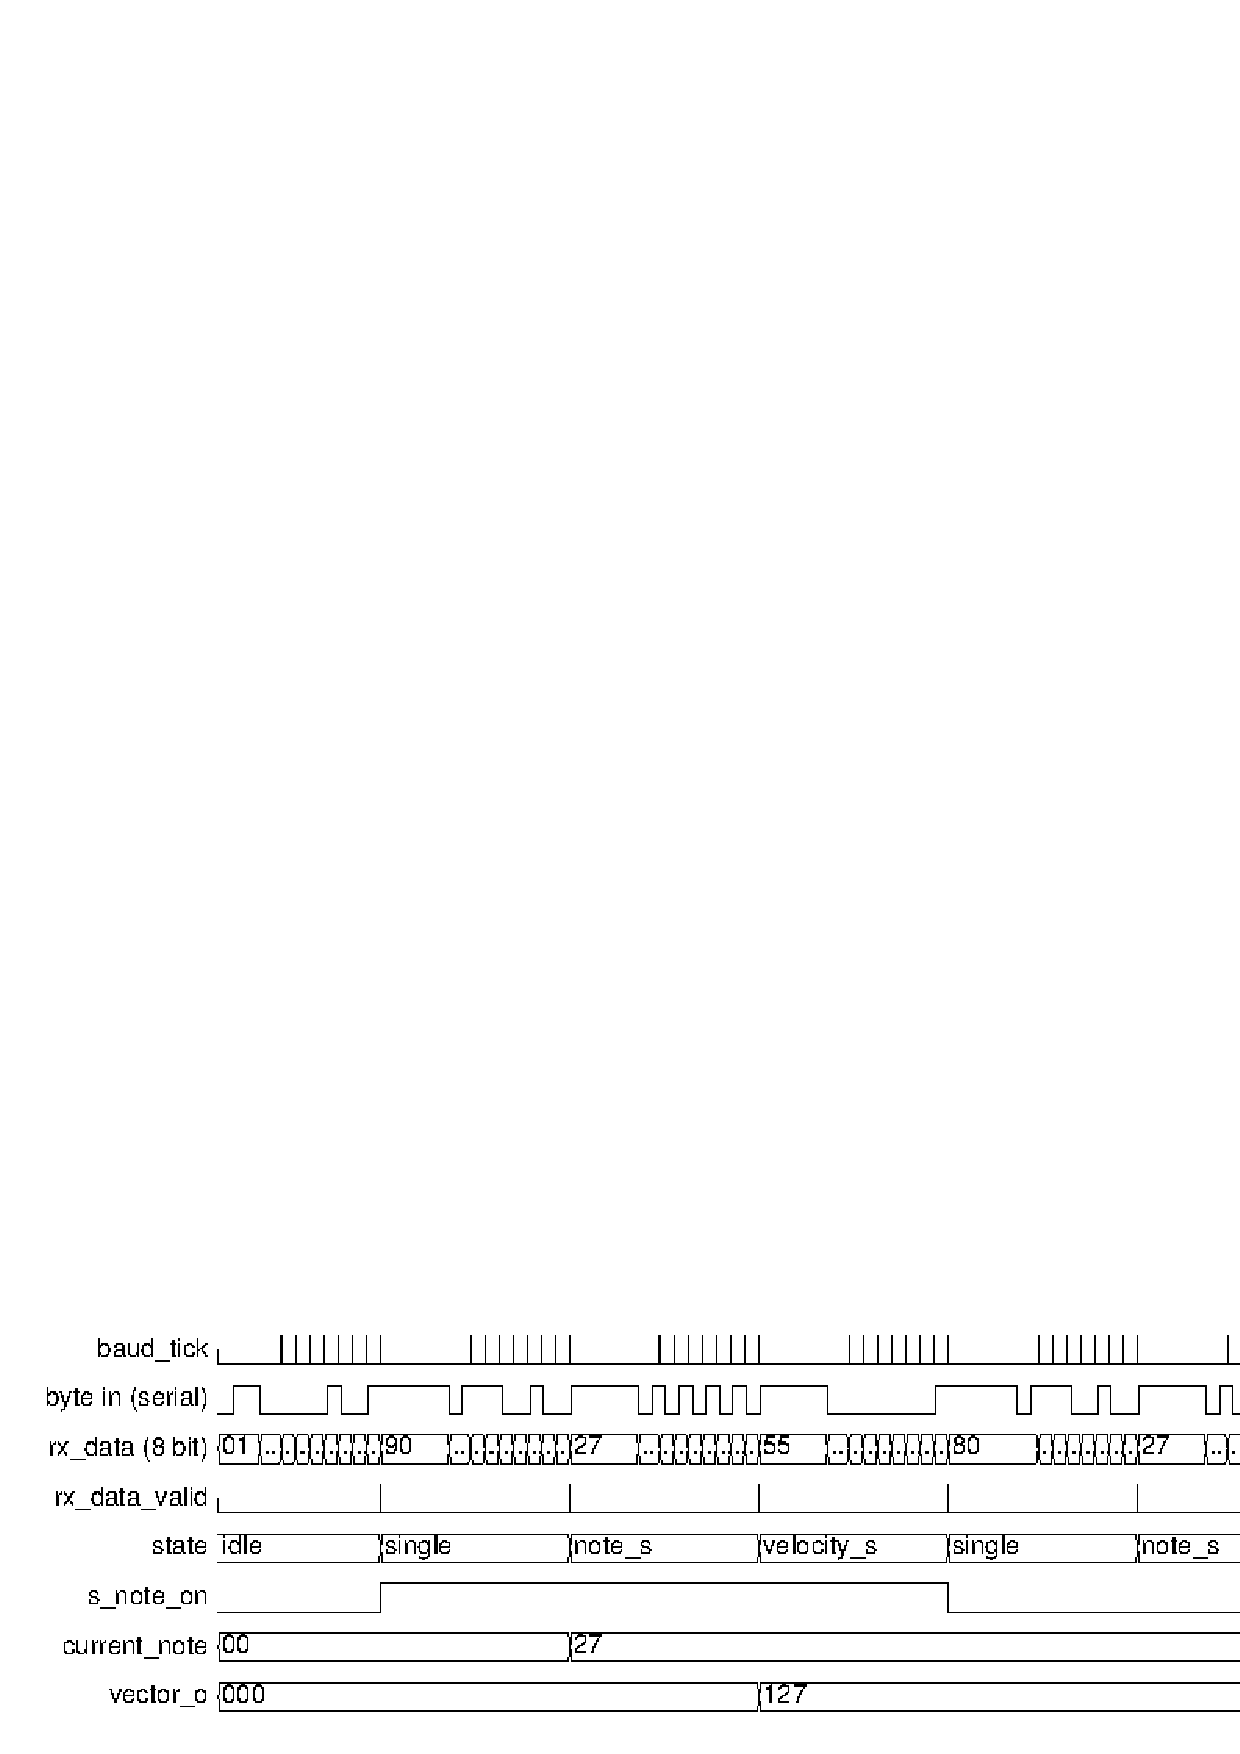
\includegraphics[width=1\textwidth]{images/midi_control/wave_single.png}
	\caption{fsm für single mode}
	\label{fig.midicontrol_singlet}
\end{figure}

\begin{itemize}
	\item Das Signal rx\_data detektiert die Befehle (0x90) und (0x80).
	\item Der Controller interpretiert  \textit{single modus}. 
	\item Die Zustandsabfolge ist korrekt: single, note\_s, velocity\_s.
	\item Zustände werden bei rx\_data\_valid = '1' die Zustände geändert.
\end{itemize}

Die Simulation zeigt, dass die Notenwerte korrekt gespeichert sind und dass das An- und Abstellen der Noten funktioniert. Am Ausgang erscheint der zusammengesetzer Vektor aus den 8 Notenbits und einem vorangestellten Bit, das detektiert, ob die aktuelle Note an oder ab ist. 



\subsection{Simulation Polyphony Mode}
\textbf{Input Daten} (Zeile 11, siehe Anhang \ref{chap.anhang_midi_input})\\
02 55 03 00 20 00 40 55 00

\textbf{Beschreibung der Befehle}\\
- Notenwert 02\\
- Note an\\
- Notenwert 03\\
- Note ab\\
- Notenwert 02\\
- Note ab\\
- Notenwert 40\\
- Note an\\

\textbf{Erwartetes Resultat}\\
Der Kontroller erkennt die Note 02, schaltet diese an und gibt am Ausgang den Vektor ''Note-02-AN'' aus. Die Note 03 wird detektiert, auf ab gesetzt und der Vektor am Ausgang zeigt ''Note-03-AB'' aus. Die nächste Note hat den Wert 2 und wird auf ab gesetzt. Der Ausgang gibt ''Note-2-Ab'' aus. Als letztes folgt die Note 40, die angestellt wird.\\

\begin{figure}[H]
	\centering
	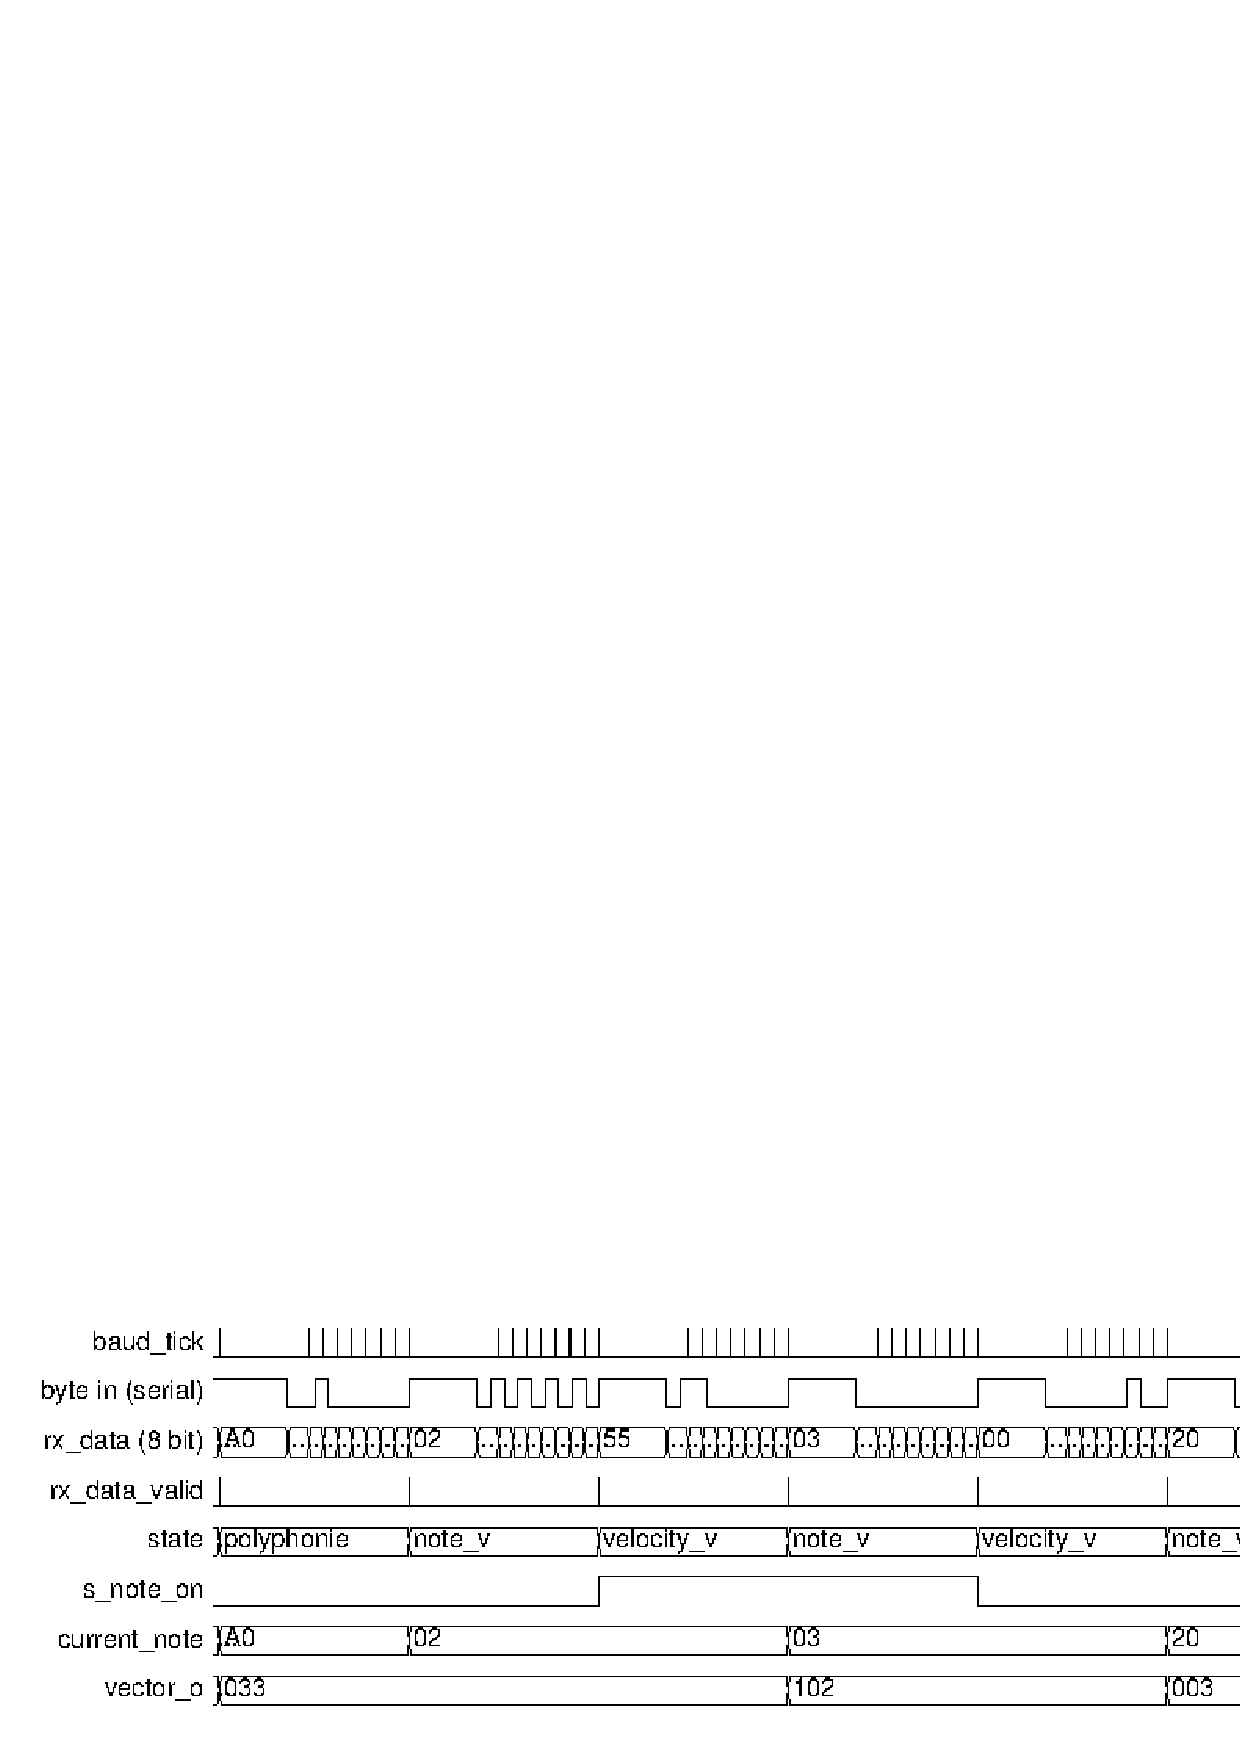
\includegraphics[width=1\textwidth]{images/midi_control/wave_polyphonie.png}
	\caption{fsm im polyphony mode}
	\label{fig.midicontrol_polyphonie}
\end{figure}


\begin{itemize}
	\item Das Signal rx\_data detektiert den Befehle (0xA0).
	\item Der Controller interpretiert  \textit{polyphony mode}. 
	\item Die Zustandsabfolge ist korrekt: polyphonie, note\_v, velocity\_v.
	\item Der Controller wartet mit dem Setzen der Note am Ausgang, bis klar ist, ob die Note an oder ab ist. \\
	Keine kurzfristig falschen Noten am Ausgang, die ab sind.
	\item Zustände werden bei rx\_data\_valid = '1' die Zustände geändert.
	\item Noten können beliebig an- und abgestellt werden
\end{itemize}


\section{Umsetzung Polyphone Out-Block}\label{sect.polyphonie_umsetzung}
 
\subsection{Funktionsbeschreibung}
Der Polyphone Out-Block speichert die empfangenen Signale in 10 Registern. Bei jeder neuen Note wird geprüft, ob der Wert im Register besteht und ob das ON/OFF-Bit der gespeicherten neu gesetzt werden muss. Der Block gibt 10 Noten parallel aus.\\

\begin{figure}[H]
	\centering
	\includegraphics[width=0.5\textwidth]{images/midi_interface/polyphonie_blockschaltbild.png}
	\caption{Polyphone Out-Block}
	\label{fig.polyphnie_out_block}
\end{figure}

\subsection{Konzept}\label{konzept_plyphonie}
Der empfangene Notenwert wird mit den gespeicherten Notenwerten verglichen. Ist eine Note vorhanden, wird das ON-OFF-Bit geprüft und aktualisiert. Keine Note darf zweimal gespeichert sein. Sind alle 10 Registerplätze besetzt, wird die neue Note in ein Register mit abgeschaltenem ON-OFF-Bit gesetzt.\\
\begin{figure}[H]
	\centering
	\includegraphics[width=0.7\textwidth]{images/midi_interface/Konzept_Hans_polyphonie.png}
	\caption{Konzept Polyphonie Block \cite{konzept_poly} }
	\label{fig.polyphnie_konzept}
\end{figure}

\subsection{Implementation}
Der Ablauf des Speicherns ist aus der Abbildung \ref{fig.polyphnie_ablauf}.
\begin{figure}[H]
	\centering
	\includegraphics[width=0.2\textwidth]{images/midi_interface/polyphnie_ablauf.png}
	\caption{Ablauf Note speichern }
	\label{fig.polyphnie_ablauf}
\end{figure}

Umgesetz wird das Suchen eines Speicherplatzes innerhalb der 10 Registern mit einer Input-Logik, die mit folgenden 3 Vergleichen arbeitet:
\begin{enumerate}
	\item Liegt der Notenwert in einem Register ? 
	\item Ist ein Register unbenützt ?
	\item Welches Register hat einen abgeschaltenen Notenwert ?
\end{enumerate}
Sobald eine Frage mit Ja beantwortet wird, wird der Registerindex gespeichert und als Output des Logik-Prozesses zur Verarbeitung weiter gegeben.\\
\newline
Durch den übermittelten Index-Wert weiss der Speicher-Prozess, in welches Register die neue Note gespeichert werden soll.\\
Die Werte aller 10 Register werden am Ausgang parallel ausgegeben.



\subsection{Resultat Polyphonie Out-Block}

\begin{figure}[H]
	\centering
	\includegraphics[width=1\textwidth]{images/midi_interface/tb_polyphonie.png}
	\caption{Simulation des Blocks Polyphonie Out }
	\label{fig.polyphnie_simulation}
\end{figure} 	
	%%%%%%%%%%%%%%%%%%%%%%%%%%%%%%%%%%%%%%%%%%%%%%%%%%%%%%%%%%%%%%%%%
%  _____       ______   ____									%
% |_   _|     |  ____|/ ____|  Institute of Embedded Systems	%
%   | |  _ __ | |__  | (___    Wireless Group					%
%   | | | '_ \|  __|  \___ \   Zuercher Hochschule Winterthur	%
%  _| |_| | | | |____ ____) |  (University of Applied Sciences)	%
% |_____|_| |_|______|_____/   8401 Winterthur, Switzerland		%
%																%
%%%%%%%%%%%%%%%%%%%%%%%%%%%%%%%%%%%%%%%%%%%%%%%%%%%%%%%%%%%%%%%%%

\chapter{Test Bench}\label{chap.testen}

\textit{Test Driven Development} bedeutet, dass vor oder parallel zur Entwicklung einer \textit{Unit} (im Folgenden Block genannt) der \textit{Unit Test} entwickelt wird \citep{Testdriven}. Beim textbasierten Testen stammen die Befehle aus einer Input-Datei, und die Ergebnisse werden in einer Datei abgelegt. 

\section{Device Under Test}\label{sec.testbench_DUT}

Das Device Under Test (DUT) ist das MIDI Interface (siehe Abbildung \ref{fig.testbench}). Das Ziel ist, dass das MIDI-Signal in den Block geführt wird und am Ausgang 10 Notenvektoren anliegen mit je 8 Notenbits und einem Bit, das besagt, ob die Note an oder ab ist.

\begin{figure}[H]
	\includegraphics[width=1\textwidth]{images/midi_interface/testbench_midiinterface.png}
	\caption{Blockschaltbild Device under Test}
	\label{fig.testbench}
\end{figure} 

Die \textit{Test Bench} wird mit Daten der Input-Datei gespiesen. Die Endversion der Input-Datei und der Testbericht liegen im Anhang \ref{chap.anhang_midi_input}. 
In den Unterkapiteln wird der Aufbau der Input-Datei, das Entwickeln der Test-Fälle, und die Umsetzung im VHDL-Code beschrieben.

\section{Struktur der Input-Datei}\label{sec.testbench_inputdatei} 

Die Test-Datei ist zeilenweise strukturiert.

\subsubsection{Verarbeitungsmodus} 

Jede Zeile beginnt mit dem Verabreitungsmodus. Bei der Input-Datei besteht der Verarbeitungsmodus aus fünf Buchstaben.

\begin{tabbing}
\hspace{4em} \= \hspace{2em} \= \hspace{2em} \=\kill
reset	\> 00 \> 00 \> \ldots{}\\
singl	\> 90 \> 27 \> \ldots{}\\
polyp	\> 71 \> 55 \> \ldots{}
\end{tabbing}

\subsubsection{Tokenstruktur} 

Nach dem Verarbeitungsmodus folgen die Daten. Jede Zeile hat gleichviele Datenpakete (Tokens). 
Die Test Bench ortet jedem MIDI-Datenpaket (siehe \ref {datentypen}, Beschreibung der MIDI-Daten) innerhalb der Zeile eine Bedeutung zu. Je nach Verarbeitungsmodus ist die Bedeutung der Token anders.

Die Tokenstruktur leitet sich aus der MIDI-Datenstruktur im Polyphony Mode und im Single Mode ab (siehe  \ref{note_modes}). In den nachfolgenden zwei Token-Beispielen bezieht sich die obere Zeile auf den Polyphony Mode und die untere auf den Single Mode.

In der \textit{Test Bench MIDI Interface} haben Tokens folgende Bedeutung:

{
\renewcommand{\arraystretch}{1.0} % avoid the extra space between the rows
\begin{tabular}{@{}*{10}{l}@{}} % @{} removes the left and right margin around the table
mode\_p	& Note & Velocity	& Note & Velocity & Note & Velocity & Note & Velocity & Anzahl Noten \\
mode\_s	& Dummy & Status & Note & Status & Note & Status & Note & Dummy & Dummy
\end{tabular}
}

Dummy ist die Bezeichnung für das Einlesen nicht relevanter Werte. Diese nicht relevanten Werte sind in der Input-Datei gesetzt, um die Verarbeitungsstruktur beim Einlesen der Token zu vereinfachen. Der Dummywert wird beim Einlesen verworfen.
 
\section{Aufstellen der Fehler}\label{sec.testbench_fehler} 

Zu Beginn hatten die Testfälle nur drei Tokens und testeten die Grundfunktionen:

single mode note an/ab\\
singl 90 27\\ 
singl 90 27

polyphone note an/ab\\
polyp 71 55\\
polyp 71 00

Komplexere Testfälle zeigten, dass eine Test-Zeile mehr Tokens braucht. Die Endversion der Input-Datei kann mit einer Zeile bis 4 Noten an und abstellen.

\subsection{Einzelne Noten testen}
 
\subsubsection{Testfälle}

Getestet sind auch Kombinationen unter den Fällen, die aus Übersichtlichkeit nicht alle aufgeschrieben werden.

\begin{itemize}
\item Einzelne Note an, Geschwindigkeit-Byte folgt
\item Einzelne Note an, Geschwindigkeit-Byte folgt nicht
\item Einzelne Note ab
\item Einzelne Note an, direkt nach Reset
\item Einzelne Note an, selbe Note nochmals an
\item Einzelne Note an, wenn in Polyphony Mode
\item Einzelne Note an, nach ungültigem Status Byte
\item Einzelne Note an, andere Note an, erste Note ab
\item Einzelne Note an, diverse andere Noten setzen, erst bei nächster Zeile erste Note ab
\end{itemize}

Zu jedem Testfall wird auf der nächsten Zeile das zu erwartende Resultat vorgegeben. Die Test Bench prüft die ausgegebene Notenwerte am Ausgang des MIDI interfaces mit den vorgegebenen Werten.

Beispielzeile\\
\rule{\textwidth}{0.4pt}\\
{
\renewcommand{\arraystretch}{1.0} % avoid the extra space between the rows
\begin{tabular*}{\textwidth}{@{}@{\extracolsep{\fill}}*{10}{l}@{}} % @{} removes the left and right margin around the table
singl & 55 & 90 & 27 & 80 & 27 & 90 & 05 & 00 & 00\\
check & 00 & 00 & 27 & 00 & 00 & 00 & 05 & 00 & 00\\
\end{tabular*}
}

Die Sequenz bedeutet Note 27 an (0x90), dann ab (0x80) der Note 27 und am Schluss an Note 05. \\
Überprüft (Check) wird, ob am Ausgang die Noten 27 und 05 anliegen.\\
Im Single Mode ist die Geschwindigkeit für das An- oder Abstellen der Note nicht relevant und wird deshalb nicht als Befehl eingelesen. Die Test Bench hängt nach jeder Note einen Dummy-Geschwindigkeitswert von 0x55 an.

\subsection{Polyphonie testen }\label{polyphonitest}

\subsubsection{Testfälle}

In der Polyphony können mehrere Noten hintereinander an- und nur einzelne davon wieder abgestellt werden.

\begin{itemize}
\item Polyphoniestatus setzen, einzelne Note an
\item Polyphoniestatus setzen, mehrere Noten an
\item Polyphoniestatus setzen, mehrere Noten über mehrere Zeilen verteilt an
\item Polyphoniestatus setzen, Note an, die bereits in Register ist
\item Polyphoniestatus setzen, Note an, andere Note an, erste Note aus, dritte Note an
\item Polyphoniestatus setzen, dritte Note aus, erste Note an, erste Note an
\item Polyphoniestatus setzen, Single Note an Status setzen, Note ohne Geschwindigkeit senden
\item Polyphoniestatus setzen, falsches Status Byte senden, Note an, Note aus,
\item Polyphoniestatus setzen, Reset, Note setzen
\item Polyphoniestatus setzen, 10 Noten an
\item Polyphoniestatus setzen, 10 Noten in Register, eine ist aus. Neue Note an senden
\end{itemize}

Beispielzeile\\
\rule{\textwidth}{0.4pt}\\
{
\renewcommand{\arraystretch}{1.0} % avoid the extra space between the rows
\begin{tabular*}{\textwidth}{@{}@{\extracolsep{\fill}}*{10}{l}@{}} % @{} removes the left and right margin around the table
polyp & 71 & 55 & 02 & 55 & 33 & 55 & 08 & 00 & 00\\
check & 71 & 00 & 02 & 00 & 33 & 00 & 00 & 00 & 03
\end{tabular*}
}

In der Sequenz wird die Note 71, dann die Noten 02 und 33. Danach wird die Note 08 abgestellt. Die Test Bench prüft am Ausgang, ob die Noten 71, 02 und 33 an sind. 

Im Verarbeitungsmodus Polyphonie sendet die Test Bench  das Status Byte \lstinline|"10100000" (0xA0)|

\section{Code Test Bench}\label{sec.code_testbench}

Die automatisierte Datenverarbeitung erzeugt viele Werte (10 Noten mit je 9 Werten). Um einzelne Bits effizient zu setzen oder zu überprüfen, wird der Code einem \textit{Refactoring} unterzogen.

Im Gegensatz zum hardwarenahen Code der VHDL-Blocks, bei denen Arrays und Loop explizit vermieden wurden, baute die Test Bench bewusst auf softwarenahe Strukturen auf.

\subsection{Package}

Damit in allen VHDL-Dateien die Arrays und Konstanten gebraucht werden können, werden diese Definitionen in einem Package zusammengefasst. Das Package kann wie eine Library zu Beginn einer VHDL-Datei eingebaut werden.
\begin{itemize}
	\item Werte der Status Bytes als Konstanten
	\item Ein- und Ausgänge als Arrays
	\item Tokenstruktur als Record
\end{itemize}

Bsp. Tokenstruktur

\begin{lstlisting}[language=vhdl]
-- define midi_data
type t_midi_data is record
    token_note : std_logic_vector(7 downto 0);
    token_attribut : std_logic_vector(7 downto 0);
    end record;

type t_midi_data_array is array (0 to 3) of t_midi_data;

-- define token structure
type t_token_line is record
    token_cmd : string(1 to 5);
    t_midi_data : t_midi_data_array;
    token_number : std_logic_vector(7 downto 0);
    end record;

-- array with note structure (input/output)
type t_note_array is array (0 to 9) of std_logic_vector(8 downto 0);
\end{lstlisting}

\subsection{Prozess-Optimierung}

Um die einzelnen Bits in den Arrays zu setzen, braucht es in der Ablaufstruktur Optimierungen.

\begin{itemize}
	\item Loops iterieren durch die Arrays
	\item Einleseprozess wird vom Verarbeitungsprozess getrennt
	\item Flags wie \lstinline|s_read_input_finished <= '1'| sichern die parallele Datenverarbeitung
\end{itemize}

\section{Ergebnisse Simulation}\label{sec.ergebnisse_tests}

Die Ausgabe der Signale in die Output-Datei bezieht sich auf den Zustand am Ausgang des DUT. Damit auch die beiden internen Blöcke MIDI Control und Polyphonie out korrekt funktionieren werden die Signale überprüft. Auch das Verhalten in den Blöcken entspricht den erwarteten Signalverläufen.

\subsection{Block Midi Control}

Gemäss der FSM durchläuft der Single Mode  die Zustände \lstinline|idle|, \lstinline|note_s|, \lstinline|velocity_s| und geht dann zurück  in den Idle-Zustand. Das Signal \lstinline|s_note_on| wechselt nach einem Status Byte von \lstinline|(0x90)| auf \lstinline|on| und nach \lstinline|(0x80)| auf \lstinline|ab|.

\begin{figure}[H]
	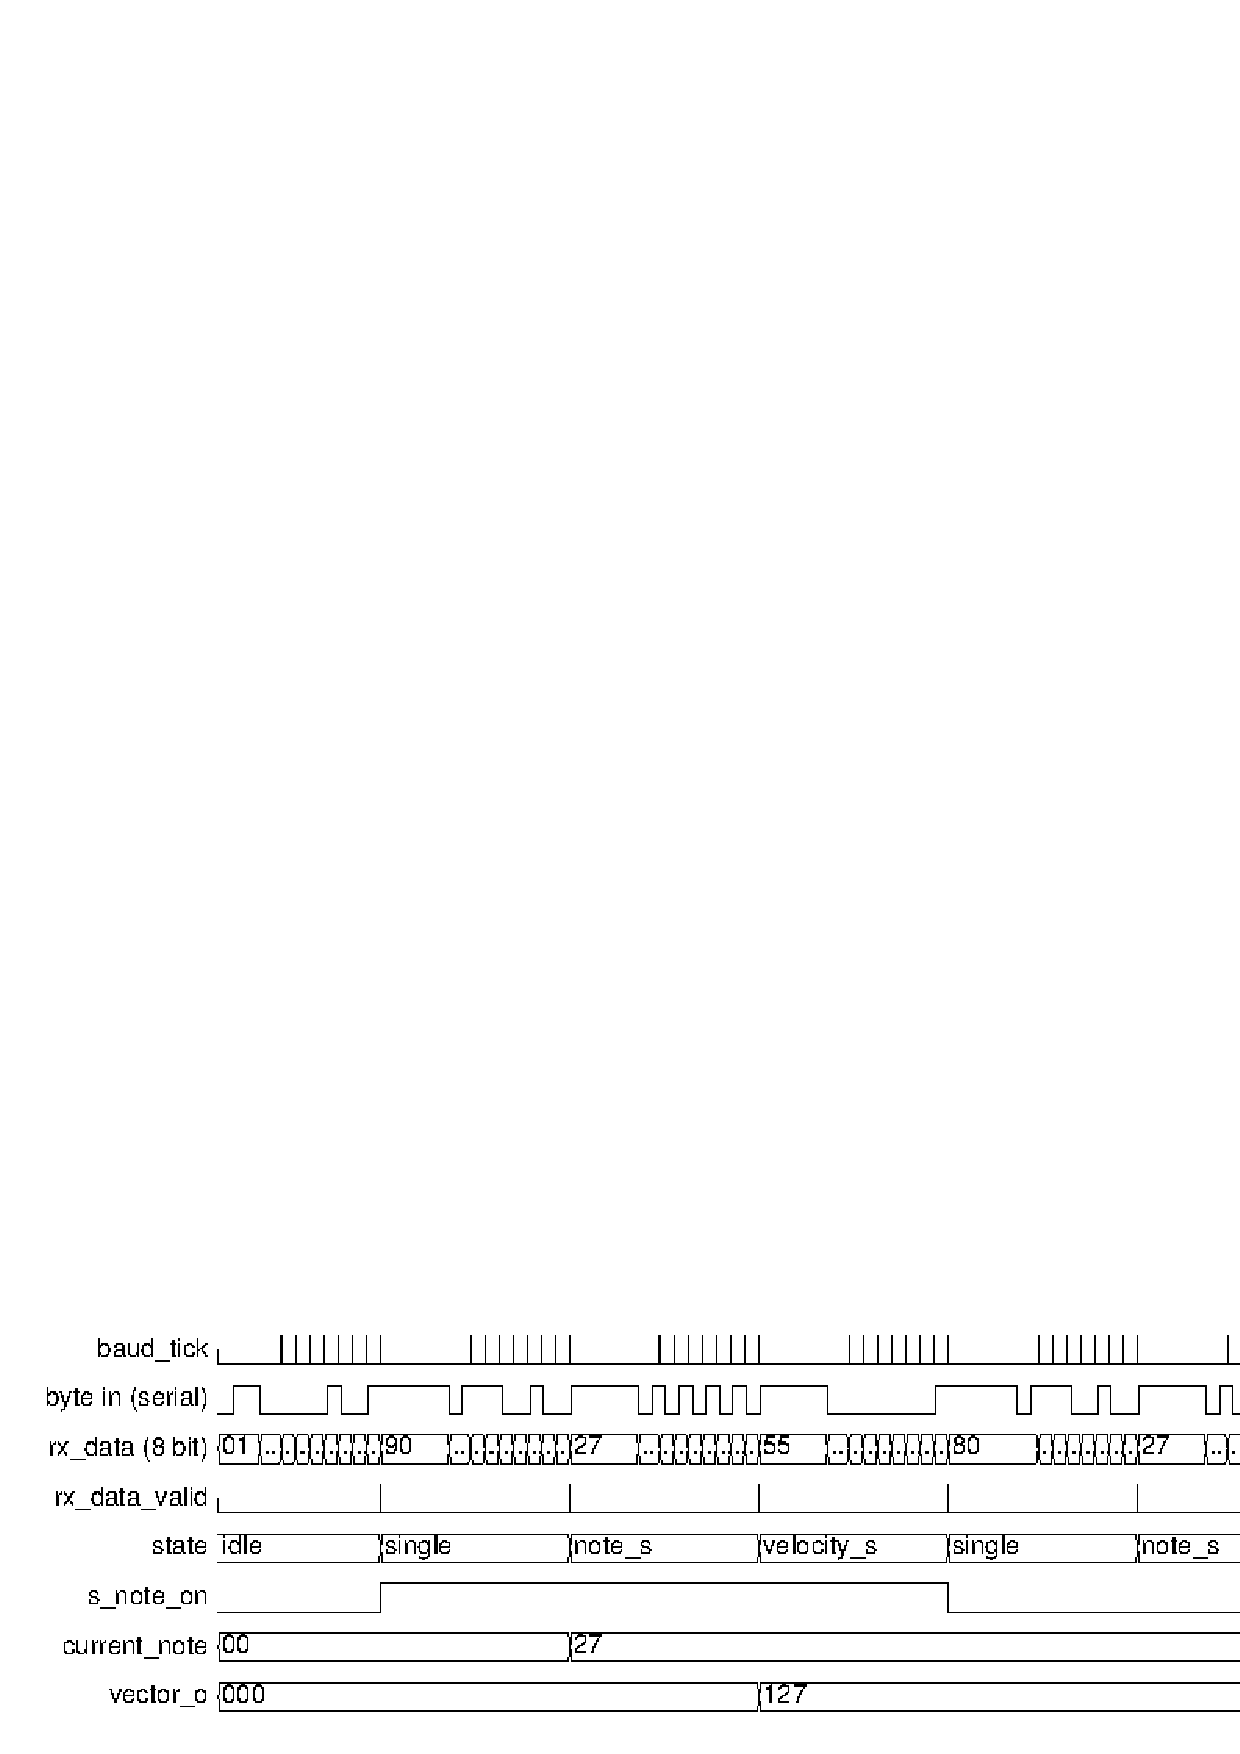
\includegraphics[width=1\textwidth]{images/midi_control/wave_single.png}
	\caption{Simulation Block Midi Control}
	\label{fig.test_midi:control_single}
\end{figure} 

Im Polyphony Mode existieren die Zustände \lstinline|idle|, \lstinline|note_v|, \lstinline|velocity_v| und verbleibt in diesem Zustand. Nur durch ein Status Byte (oder ungültige Data Bytes) wird der Zustand der Polyphonie verlassen.

\begin{figure}[H]
	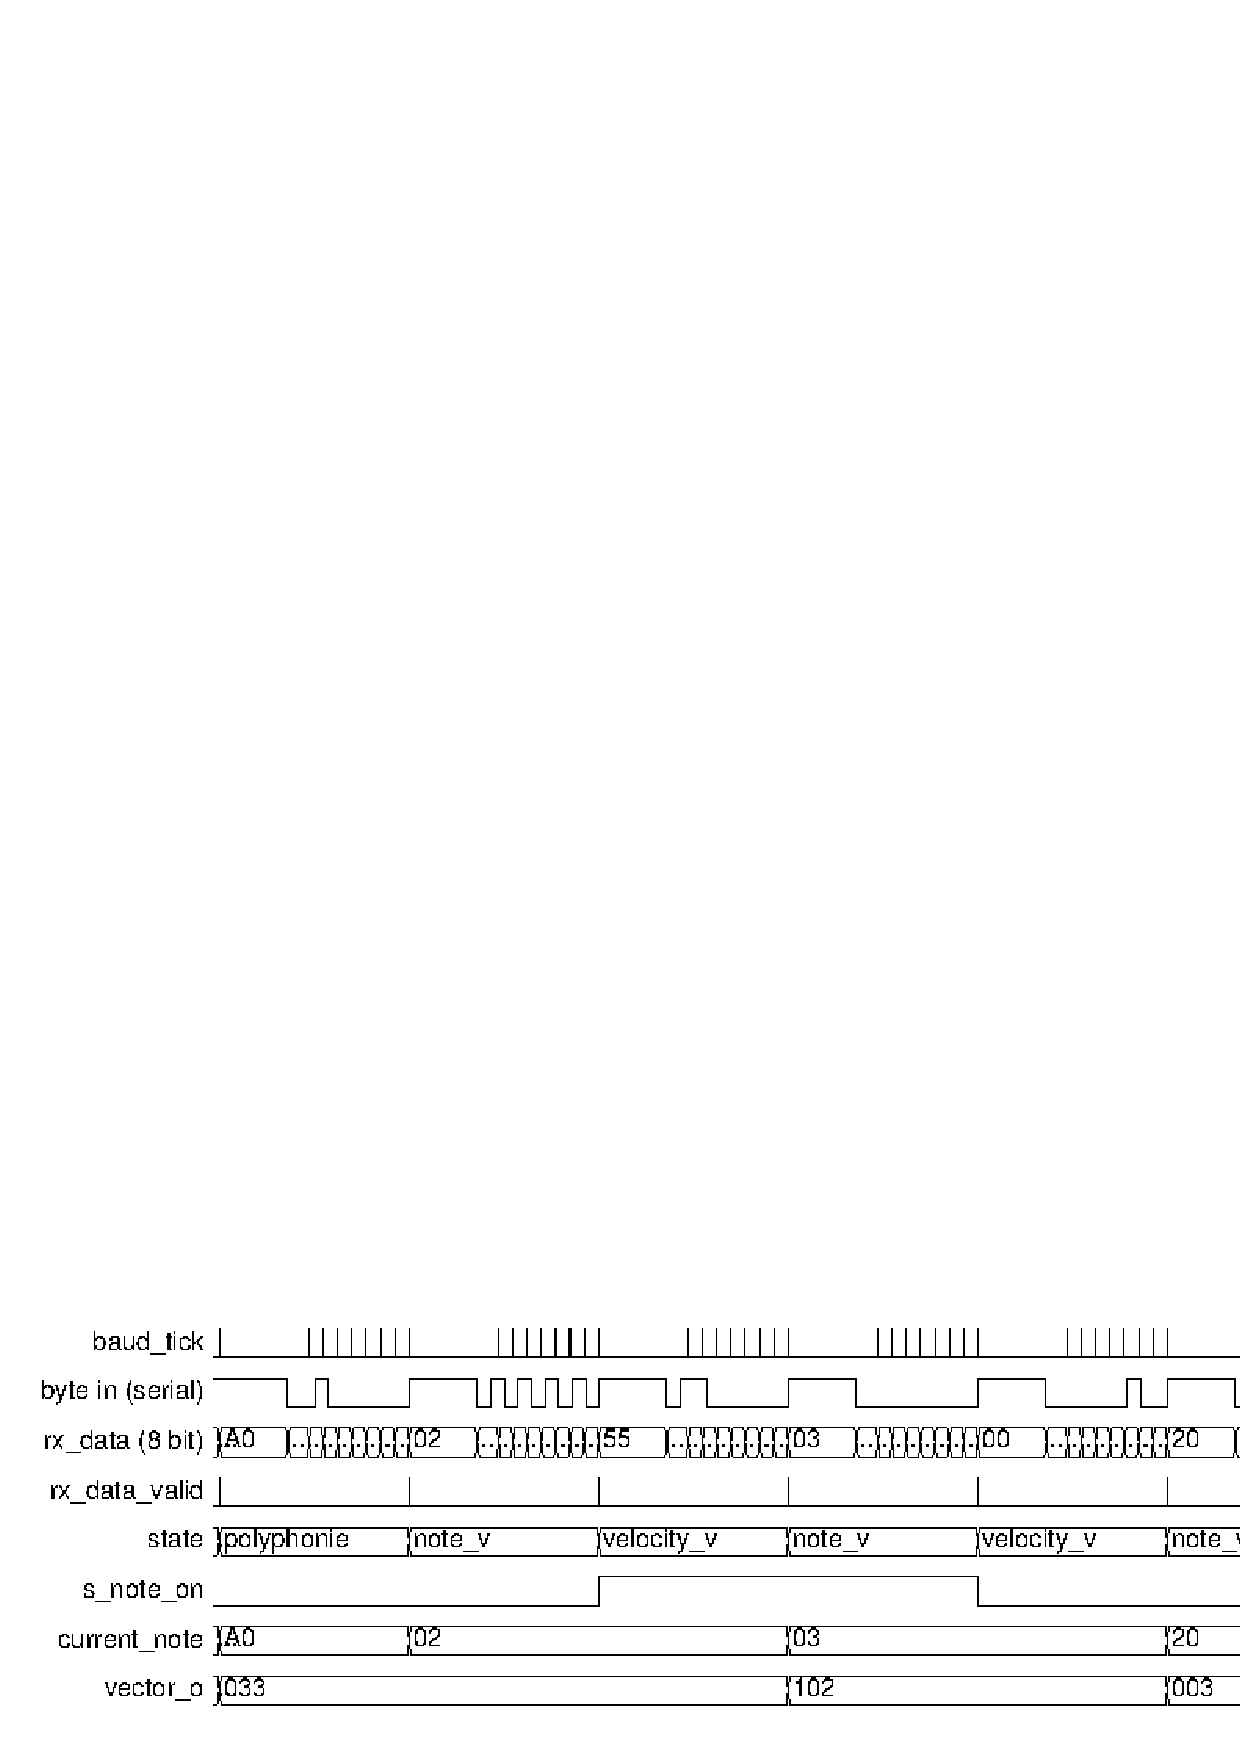
\includegraphics[width=1\textwidth]{images/midi_control/wave_polyphonie.png}
	\caption{Simulation Block Midi Control}
	\label{fig.test_midi:control}
\end{figure} 

\subsection{Block Polyphony Out}

Kriterien in der Polyphonie out sind, dass jede neue Note auf den nächsten freien Register-Platz gelegt wird. Zudem soll keine Note zwei Registerplätze belegen. Zudem soll, wenn alle Register-Plätze einen Notenwert haben, die neue Note an einen Registerplatz mit aktuell abgeschalteter Note besetzen.\\
Alle Kriterien (siehe \ref {test_polypohnie}) sind erfüllt.

\begin{figure}[H]
	\includegraphics[width=1\textwidth]{images/midi_interface/tb_polyphonie.png}
	\caption{Simulation Block Polyphony Out}
	\label{fig.test_polyphonie}
\end{figure} 

	%%%%%%%%%%%%%%%%%%%%%%%%%%%%%%%%%%%%%%%%%%%%%%%%%%%%%%%%%%%%%%%%%
%  _____       ______   ____									%
% |_   _|     |  ____|/ ____|  Institute of Embedded Systems	%
%   | |  _ __ | |__  | (___    Wireless Group					%
%   | | | '_ \|  __|  \___ \   Zuercher Hochschule Winterthur	%
%  _| |_| | | | |____ ____) |  (University of Applied Sciences)	%
% |_____|_| |_|______|_____/   8401 Winterthur, Switzerland		%
%																%
%%%%%%%%%%%%%%%%%%%%%%%%%%%%%%%%%%%%%%%%%%%%%%%%%%%%%%%%%%%%%%%%%

\chapter{Diskussion und Ausblick}\label{chap.diskussion}

Bespricht die erzielten Ergebnisse bezüglich ihrer ERwartbarkeit, Aussagekraft und Relevanz\\
Interpretation und Validierung der Resultate\\
Rückblick auf Aufgabenstellung: erreicht\ nicht erreicht\\

Legt dar, wie die Resultate weiterhin genutzt werden können\\ an sie angeschlossen werden kann\\




% Aus derr Einleitung
Als offener Punkt besteht die Implementation des \textit{midi interfaces} in das bestehende Synthesizer-Projekt. Die Schnittstellen sind im Anhang festgehalten und die notewnigen Implementationsschritte, wie das Ausweiten des bestehenden DDS auf 10 DDS sind im Projekt als Blöcke eingebaut. Aus zeitlichen Gründen konnte dieser letzte Schritt nicht mehr während der Projektarbeit zu Ende gebracht werden. 
	%%%%%%%%%%%%%%%%%%%%%%%%%%%%%%%%%%%%%%%%%%%%%%%%%%%%%%%%%%%%%%%%%
%  _____       ______   ____									%
% |_   _|     |  ____|/ ____|  Institute of Embedded Systems	%
%   | |  _ __ | |__  | (___    Wireless Group					%
%   | | | '_ \|  __|  \___ \   Zuercher Hochschule Winterthur	%
%  _| |_| | | | |____ ____) |  (University of Applied Sciences)	%
% |_____|_| |_|______|_____/   8401 Winterthur, Switzerland		%
%																%
%%%%%%%%%%%%%%%%%%%%%%%%%%%%%%%%%%%%%%%%%%%%%%%%%%%%%%%%%%%%%%%%%

\chapter*{Verzeichnis}\label{chap.verzeichnis}

\section{Literaturverzeichnis}\label{sect.verzeichnis_literatur}
%\renewcommand{\section}[1]{} %verhindert neue section
%\bibliographystyle{abbrvnat}
%\setcitestyle{authoryear,open={(},close={)}})
\bibliography{BibTex/references}



%\section{Bildverzeichnis}\label{sect.verzeichnis_bilder}
%\section{Glossar}\label{sect.verzeichnis_glossar}

\textbf{Durchlaufverzögerung}\\
Wird englisch \textit{propagation delay} genannt und bezeichnet die Zeit, die Daten vom Eingang bis zum Ausgang des Bauteils brauchen.\\
Die Durchlaufverzögerung beträgt beim Cylone IV 4 ns (Device Handbook, S. 8-19).\\


\textbf{hold time}\\
Ist die minimale Zeit, in der die Inputdaten \textit{nach} der Taktflanke stabil sein müssen.\\
Die hold-Zeit beträgt beim  Cyclone IV E 0 ns (Device Handbook, S. 8-19).\\


Pfadzeit\\
... (Unter 3.2. Metastabilität Ratschläge erwähnt)\\



\textbf{quartus}\\
IDE von altera zum Kompilieren, Synthesizieren und einbauen von IPs für die altera FPGAs.\\


\textbf{setup time} \\
minimale Zeit, in der Inputdaten stabil sein müssen be\textit{vor} ein Taktflanke die Daten triggert.\\
Die setup-Zeit beträgt beim Cyclone IV E 10 ns (Device Handbook, S. 8-19)\\





	%%%%%%%%%%%%%%%%%%%%%%%%%%%%%%%%%%%%%%%%%%%%%%%%%%%%%%%%%%%%%%%%%
%  _____       ______   ____									%
% |_   _|     |  ____|/ ____|  Institute of Embedded Systems	%
%   | |  _ __ | |__  | (___    Wireless Group					%
%   | | | '_ \|  __|  \___ \   Zuercher Hochschule Winterthur	%
%  _| |_| | | | |____ ____) |  (University of Applied Sciences)	%
% |_____|_| |_|______|_____/   8401 Winterthur, Switzerland		%
%																%
%%%%%%%%%%%%%%%%%%%%%%%%%%%%%%%%%%%%%%%%%%%%%%%%%%%%%%%%%%%%%%%%%


\pagenumbering{Roman}

\appendix
\chapter{Anhang: Englische Definitionen Glitches}\label{chap.anhang_dictionaire}
%\begin{quote}A sudden, usually temporary malfunction or irregularity of equipment\end{quote},
 %oxford Dictionaries, (oxforddictionaries.com \textslach{de}\textslach{defintion}\textslach {englischusa}\textslach{glitch, 11.okt.2015)}\\
 
 
%\newline
%\begin{quote}A ​sudden ​unexpected ​increase in ​electrical ​power, ​especially one that ​causes a ​%fault in an ​electronic ​system\end{quote}, %http://dictionary.cambridge.org/de/worterbuch/englisch/glitch\\
%\newline

%\begin{quote}The \textit{glitch} is that unwanted \textit{spike} or transient output that increments some counter, clears some register, or starts some unwanted process at precisely the most undesirable time. This transient an undesirable spike is generally issued form any decoder that is addressed with a sequence of NON-UNIT-DISTANCE-CODED inputs.\end{quote}(Fletcher, Digital design, 472).\\





\newpage
\chapter{Anhang: VHDL-Code Glitch detect }\label{chap.anhang_2.vhdl_glitch}
%-------------------------------------------------------------------------------
%-- Project     : Glitches detect through long logic paths
%-- Description : glitch_detection.vhd    
%-- 				: Detect value 15. Once asynchronous (= glitch), once synchronous (cnt)         
%-- Author      : Katrin Bächli
%-------------------------------------------------------------------------------
%-- Change History
%-- Date     |Name      |Modification
%------------|----------|-------------------------------------------------------
%-- 05.10.15	| baek     | init
%-- 06.10.15 | baek     | add cnt-singal and clock
%-------------------------------------------------------------------------------
%
%
%library ieee;
%use ieee.std_logic_1164.all;
%use ieee.numeric_std.all;
%
%
%entity glitch_detection is
%	port(	clk: 				in std_logic;
%			glitch:			out std_logic; 
%			count:			out std_logic;	
%			-- Routing
%			q_0_out:			out std_logic;
%			q_1_out:			out std_logic;
%			q_2_out:			out std_logic;
%			q_3_out:			out std_logic;
%			------
%			q_0_in:			in  std_logic;
%			q_1_in:			in  std_logic;
%			q_2_in:			in  std_logic;
%			q_3_in:			in  std_logic
%	);
%end entity;
%
%
%
%architecture rtl of glitch_detection is 
%
%----------------------------------------------------------------------------------
%-- signal
%----------------------------------------------------------------------------------
%
%signal  cnt_async: 		integer range 0 to 15 		  := 0;
%signal  next_cnt_async: integer range 0 to 15 		  := 0;
%signal  detect_15_async: std_logic 						  := '0';  
%
%signal  cnt_sync:			std_logic						  := '0';
%signal  cnt_sync_next:	std_logic						  := '0';  
%
%
%signal  rout_out:       std_logic_vector(7 downto 0) := "00000000";
%signal  rout_in:        std_logic_vector(7 downto 0) := "00000000";
%
%
%
%begin
%
%------------------------------------------------------
%-- input
%------------------------------------------------------	
%		
%	count_up: process(ALL)	
%	begin
%		next_cnt_async <= cnt_async + 1;
%	end process;
%
%	
%------------------------------------------------------
%-- clocked processes
%------------------------------------------------------	
%	ff: process(clk)	
%	begin			
%		if (rising_edge(clk)) then		
%				cnt_async 		<= next_cnt_async;
%				cnt_sync 		<= cnt_sync_next;					
%		end if;
%	end process;
%
%	
%------------------------------------------------------
%-- delay
%------------------------------------------------------
% 
%	rout_out <= std_logic_vector(to_unsigned(cnt_async, 8));
%   q_0_out  <=  rout_out(0);   
%   q_1_out  <=  rout_out(1);
%   q_2_out  <=  rout_out(2);
%   q_3_out  <=  rout_out(3);  
%   ------------------
%	rout_in(0)	  <=  q_0_in;   
%   rout_in(1)	  <=  q_1_in;
%   rout_in(2)	  <=  q_2_in;		
%		
%		
%------------------------------------------------------
%-- output
%------------------------------------------------------	
%	
%	reset_counter: process(ALL)	
%	begin	
%	   -- asynchronous
%		if ( rout_in(0) = '1' AND rout_in(1) = '1' AND rout_out(2) = '1' AND rout_out(3) = '1') then  
%			detect_15_async <= '1';
%			cnt_sync_next <= '1';
%		else 
%			detect_15_async <= '0';
%			cnt_sync_next <= '0';
%		end if;	
%	end process;
%		
%	-- set outputs
%	count  <= cnt_sync;
%	glitch <= detect_15_async;
%
%end rtl;





\newpage
\chapter{Anhang: VHDL-Code Metastability detect }\label{chap.anhang_2.vhdl_metastability}
%library IEEE;
%use IEEE.STD_LOGIC_1164.ALL;
%use IEEE.NUMERIC_STD.ALL;
%
%ENTITY metastability_2 IS
%
%port (CLOCK_27 : 	in std_logic;
%		CLOCK_50 : 	in std_logic;
%		KEY_1 : 		in std_logic; 		-- reset-button
%      GPIO_0_0 :  out std_logic;		-- KO: state 
%		GPIO_0_1 :  out std_logic;    -- KO: async. pulse 
%		SW_17:      in std_logic;     -- synchronisation-switch
%		LEDR_0:		out std_logic;
%		LEDR_1:		out std_logic;
%		LEDG_7:		out std_logic			
%  );
%end metastability_2; 
%
%
%----------------------------------------------------------------------------------
%-- Architecture 
%----------------------------------------------------------------------------------
%architecture behavioral of metastability_2 is
%
%--------------------------------------------
%-- Signals and Constants
%--------------------------------------------
%constant s0			: std_logic_vector(2 downto 0) := "001";
%constant s1 		: std_logic_vector(2 downto 0) := "010";
%constant unstable : std_logic_vector(2 downto 0) := "000";
%
%signal state: 			std_logic_vector(2 downto 0);  
%signal next_state: 	std_logic_vector(2 downto 0);
%
%signal cnt: 			integer range 0 to 15 := 0;  
%signal next_cnt: 		integer range 0 to 15 := 0; 
%signal cnt_reset:		std_logic     := '0'; 
%
%signal pulse_async: 	std_logic     := '0';
%signal pulse_sync1: 	std_logic     := '0';
%signal pulse_sync2: 	std_logic     := '0';
%signal pulse: 			std_logic     := '0';
%
%
%begin
%
%--------------------------------------------
%-- Clocked Process
%--------------------------------------------
%	fsm: process (all)
%	begin
%		if (KEY_1 = '0') then
%			state <= s0;
%		elsif (rising_edge(CLOCK_50)) then
%		   state <= next_state;
%			-- synchronistaion of async. pulse
%		   pulse_sync1 <= pulse_async;
%		   pulse_sync2 <= pulse_sync1;
%		end if;
%	end process;
%
%
%	counter: process (all)
%	begin
%		if (KEY_1 = '0') then
%			cnt <= 0;
%		elsif(rising_edge(CLOCK_27)) then
%		   cnt <= next_cnt;   			
%		end if;
%	end process;
%	
%
%	
%--------------------------------------------
%-- Asynynchronous Pulse Counter
%-------------------------------------------- 
%	counter_input: process (all)	
%	begin			
%			next_cnt <= cnt + 1; 
%	end process;
%
%	
%--------------------------------------------
%-- Test Metastable State Machine Logic
%-------------------------------------------- 	
%	fsm_input: process (all)		
%	begin 	
%	  case state is
%	  	 when s0 => 
%			 if(pulse ='1') then
%				 next_state <= s1;
%			 else
%				 next_state <= s0;
%			 end if;  
%			
%		 when s1 =>    
%			 if(pulse ='1') then
%				 next_state <= s0;
%			 else
%				 next_state <= s1;
%			 end if;
%			 
%		 when others => 
%				next_state <= unstable;
%				
%	  end case;		
%end process;	
%
%--------------------------------------------
%-- Synchronisation by Switch
%--------------------------------------------
%	multiplexer_synchro: process (all)
%	begin
%		if (SW_17 = '1') then
%			pulse <= pulse_sync2;
%		else 
%			pulse <= pulse_async;
%		end if;
%	end process;
%	
%
%--------------------------------------------
%-- Output Process
%--------------------------------------------
%
%	decode_cnt_max: process (all)
%	begin
%		if (cnt = 15) then
%			pulse_async <= '1';
%		else 
%			pulse_async <= '0';
%		end if;
%	end process;	
%
%	
%	fsm_output: process (all)
%	
%	begin
%	
%	-- Default Values
%	LEDR_0   <= '0';
%	LEDR_1   <= '0';
%	LEDG_7   <= '0';  
%	GPIO_0_0 <= '0';
%	
%		case state is
%			when s0 =>   
%					LEDR_0  <= '1'; 
%			when s1 =>   
%					LEDR_1  <= '1'; 
%					GPIO_0_0 <= '1';
%			when unstable => 
%			      LEDG_7  <= '1';
%			when others =>   
%					LEDG_7 <= '1';		 
%		end case;			
%	end process;	
%	
%   -- Set Output	
%	GPIO_0_1 <= pulse_async;
%	
%end behavioral;




\section{Bliblibli}\label{sect.anhang.ah}



\begin{itemize}
	\item sfasdfasdfasfasf
\end{itemize}
\newpage
	
	

	

\end{document}
%---------------------------------------------------------------------
